\section{Problem 1}
To build an ARIMA model for the given data, I first inspect the time plot of the data, which given on top of Figure \ref{fig:mkts}. Obviously, the data is not stationary. There is an obvious trend, and the variance seems to increase over time. This suggests that we should use log transformation to first stabilize the variance. The time series after taking log is shown in the middle of Figure \ref{fig:mkts}. We see that the variance is now more stable, but the trend is still there. Therefore, I try to differentiate the log of mkts to detrend the series. The result is shown in the bottom of Figure \ref{fig:mkts}. I now refer to the differentiated log of mkts time series as mkgr, which is the quarterly growth rate of mkts. The time plot of mkgr shows that the time series is now relatively stable without any obvious trend. However, we can see that there seems to be different periods where the variances are significantly different. The time series variance is very large during 1980 to around $1992$. From 1993 to around 2007, the time series variance becomes very small. After 2008, the variance seems to increase again. This suggests that there could be a hidden state switching between those periods. I ignore those facts for now, and try to build an ARIMA model for the mkgr time series.

We now look at the sample ACF and PACF to identify appropriate autoregressive order $p$ and the moving average order $q$ for the ARIMA model. The plot is given in Figure \ref{fig:acf}. We see that the PACF is cutting off at lag 3, and the ACF is tailing off without any strong seasonal pattern. This suggests an AR(3) model. I also try an ARIMA(3,0,1) to see if an extra moving average term can help in this case. After fitting the two models, I get the result that ARIMA(3, 0, 0) has a smaller BIC score. However, the AIC and AICc both prefer the ARIMA(3, 0, 1) model. In this case, I choose the model ARIMA(3, 0, 0) to work on, since a simple model is probably more easily to be interpreted.

The estimated ARIMA(3, 0, 0) model is:
\begin{equation}
x_t = .0154_{(.0091)} + -.6277_{(.0766)} x_{t-1} -.4534_{(.0840)}- .3261_{(.0760)} + \hat{w}_t
\end{equation}
where $\hat{\sigma}_w = 0.0714$
\begin{figure}
	\centering
	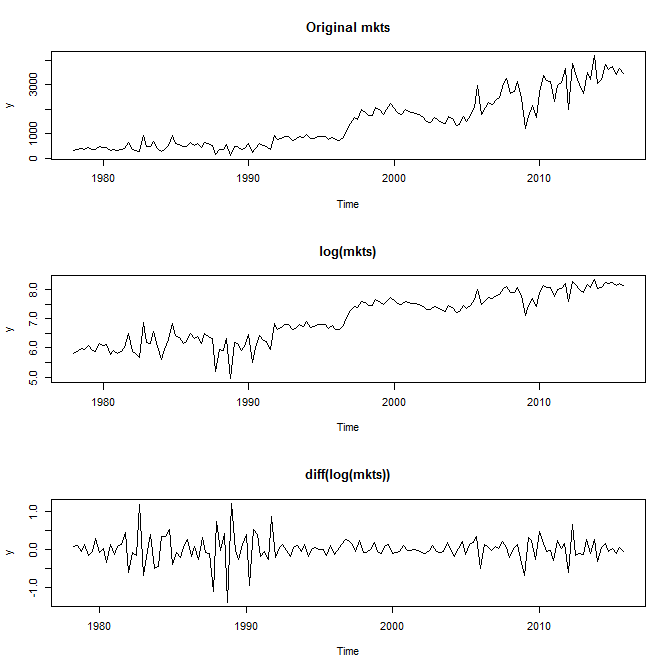
\includegraphics[width=10cm]{Figures/Problem1_mkts}
	\caption{\emph{Top:} time plot of the original mkts data. \emph{Middle:} mkts after taking log. \emph{Bottom:} mkts after differencing log}
	\label{fig:mkts}
\end{figure}
\begin{figure}
	\centering
	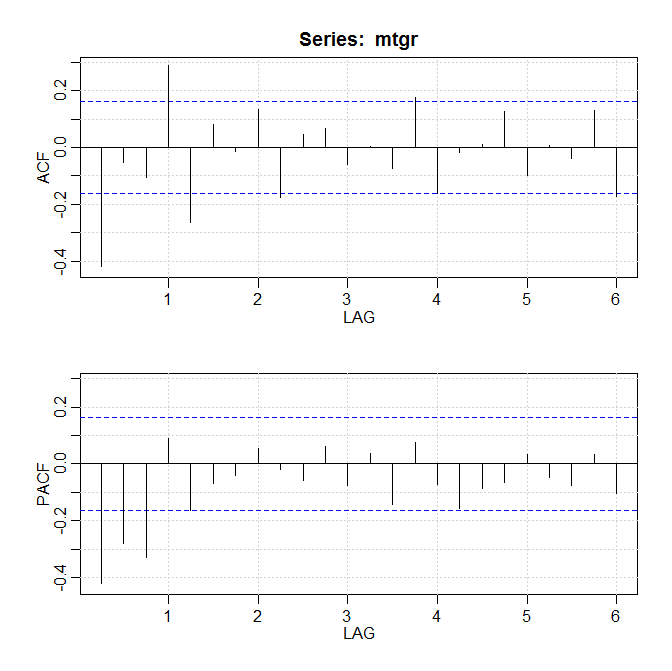
\includegraphics[width=10cm]{Figures/Problem1_acf}
	\caption{The sample ACF and PACF of the mkgr series. Lag is in terms of years.}
	\label{fig:acf}
\end{figure}
\subsection{Diagnostics for the fitted ARIMA(3, 0, 0) }
The plot of the ARIMA(3, 0, 0) residuals, its sample autocorrelation function, Q-Q plot, and Q-statistic are given in Figure \ref{fig:residual}. From the time plot of the standardized residuals, we see that there are 3 periods that have significant difference in variance, as indicated previously. Other than that, there is no obvious patterns. The residuals' ACF plot confirms this argument, as there is not significant correlation in the residuals time series. The Q-statistic tells the same story, which is never significant in the plot. The Q-Q plot shows that the residuals departure from normality at the tails due to outliers during the high variance periods. In general, the model fit the data pretty well, with the only problem is the difference in variance during different periods, which leads to fat tails of residuals distribution.

\begin{figure}
	\centering
	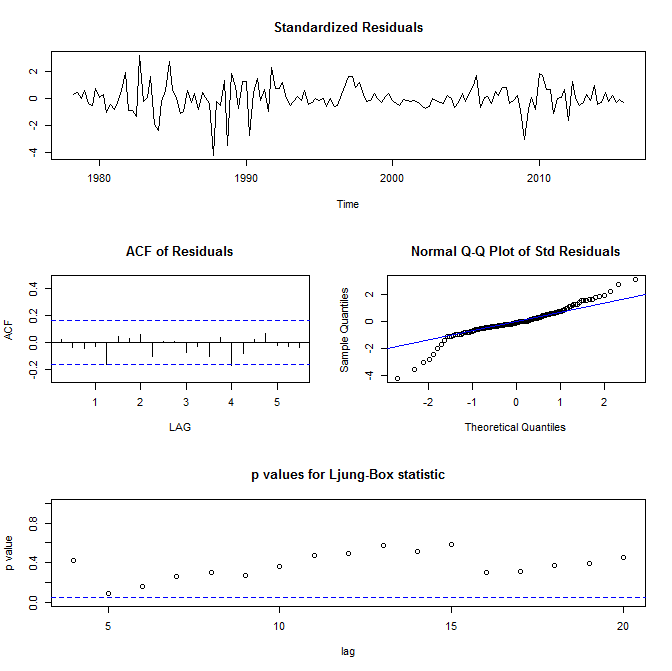
\includegraphics[width=10cm]{Figures/Problem1_residual}
	\caption{Diagnostics of the residuals from ARMA(3,0,0) fit on mkgr}
	\label{fig:residual}
\end{figure}

\subsection{Forecasting}
The forecast for the next two year of the mkts series using the above model is given in Figure \ref{fig:forecast}. Note that the figure is given in log scale.
\begin{figure}
	\centering
	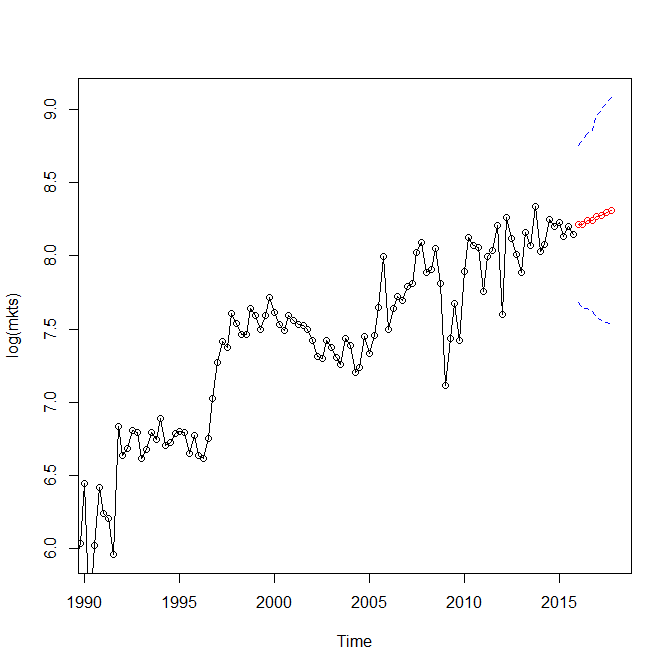
\includegraphics[width=10cm]{Figures/Problem1_forecast}
	\caption{Forecast for the next two year of log of the mkts series}
	\label{fig:forecast}
\end{figure}